\documentclass[a4paper, 12pt]{book}

\usepackage[paperwidth=22.3cm, paperheight=22.3cm, asymmetric, twoside,
bindingoffset=0.76cm, inner=1.27cm, outer=1.27cm, top=1.27cm,
bottom=2.17cm, marginparwidth=0cm,noheadfoot, nomarginpar]{geometry}

\bibliographystyle{unsrt}

\setlength{\footskip}{3\baselineskip}

\PassOptionsToPackage{unicode}{hyperref}
\IfFileExists{footnotehyper.sty}{\usepackage{footnotehyper}}{\usepackage{footnote}}
\IfFileExists{xurl.sty}{\usepackage{xurl}}{} % add URL line breaks if available
\usepackage{graphicx}
\usepackage{amsmath,amssymb,amsthm}
\usepackage{longtable,booktabs,array}
\usepackage{calc} % for calculating minipage widths
\usepackage[T1]{fontenc}

\usepackage[dvipsnames]{xcolor}
\usepackage{pagecolor}
\usepackage{anyfontsize}
\usepackage[most]{tcolorbox}
\usepackage[german]{babel}
\usepackage{multicol}
\usepackage{fancyhdr}
\usepackage{wrapfig}
\usepackage{xparse}
\usepackage{listofitems}
\usepackage[symbol*]{footmisc}
\usepackage[colorlinks=true,urlcolor=.,linkcolor=.]{hyperref}
\usepackage{imakeidx}
\usepackage{mathtools}

\makeindex[title={Index}]

% page numbers...
\tcbset{on line,
        boxsep=4pt, left=0pt, right=0pt, top=0pt, bottom=0pt,
        colframe=orange!50, colback=orange, highlight math style={enhanced}}
\fancypagestyle{plain}{
\fancyhf{} % clear all header and footer fields
\fancyfoot[EC,OC]{
\raisebox{\height}{
% \tcbox{\;\textcolor{white}{\thepage}\;}}
 \thepage
}
}
\renewcommand{\headrulewidth}{0pt}
\renewcommand{\footrulewidth}{0pt}}

\pagestyle{plain}

\pagecolor{white}

% fonts...
\usepackage[sfdefault]{roboto}
\usepackage{fontspec}
\setmainfont[Mapping=tex-text]{Roboto}
\setsansfont[Mapping=tex-text]{Roboto}
\setmonofont[Mapping=tex-text, Scale=1]{Courier New Bold}
\newfontfamily\titlefont[Mapping=tex-text]{Roboto}
\newfontfamily\sectiontitlefont[Mapping=tex-text]{Roboto}

\usepackage{amsmath}
\usepackage{unicode-math}
\setmathfont{Fira Math}
\setmathfont[range=up]{Roboto}
\setmathfont[range=it]{Roboto-Italic}
\setmathfont[range=\int]{Fira Math}

% paragraphs...

\parskip5pt
\parindent0pt

% for images...

\ExplSyntaxOn
\NewDocumentCommand{\aspectratio}{smo}
 {% #2 is the image file
  \hbox_set:Nn \l_tmpa_box {\includegraphics{#2}}
  \IfNoValueTF{#3}
   {
    \__student_aspectratio:nn { \box_wd:N \l_tmpa_box } { \box_ht:N \l_tmpa_box }
   }
   {
    \IfBooleanTF{#1}{ \tl_gset:Nx } { \tl_set:Nx } #3
     {
      \__student_aspectratio:nn { \box_wd:N \l_tmpa_box } { \box_ht:N \l_tmpa_box }
     }
   }
 }

\cs_new:Nn \__student_aspectratio:nn
 {
  \fp_eval:n {round( #1 / #2 , 5)}
 }
\ExplSyntaxOff

% templates...

\newsavebox{\storytext}

\newcommand{\PhotoTextC}[3]{ % centered photo+text: image, text, page bgcolor
\savebox{\storytext}{\parbox[b]{\textwidth}{#2}}
\begin{center}
% Compute height (subtract another 20pt to make sure that the text fits, this is hardcoded, FIXME):
\includegraphics[height={\dimexpr\textheight-\ht\storytext-20pt\relax}]{#1}

#2
\end{center}
\pagecolor{#3}
\newpage
\pagecolor{white}
} % \PhotoTextC

\newcommand{\PhotoTextJ}[4]{ % justified photo+text: photo width, image, text, page bgcolor
\begin{center}
 \includegraphics[width=#1\linewidth]{#2}
\end{center}

#3
\pagecolor{#4}
\newpage
\pagecolor{white}
} % \PhotoTextJ

\newcommand{\TextJPhoto}[4]{ % justified text+photo: text, photo width, image, page bgcolor
#1

\begin{center}
 \includegraphics[width=#2\linewidth]{#3}
\end{center}

\pagecolor{#4}
\newpage
\pagecolor{white}
} % \TextJPhoto



\newcommand{\PhotoTextJPhoto}[6]{ % justified photo+text+photo: photo width, image, text, photo width, image, page bgcolor
\begin{center}
 \includegraphics[width=#1\linewidth]{#2}
\end{center}

#3

\begin{center}
 \includegraphics[width=#4\linewidth]{#5}
\end{center}
\pagecolor{#6}
\newpage
\pagecolor{white}
} % \PhotoTextJPhoto


\newcommand{\PhotoTextCPhoto}[6]{ % centered photo+text+photo: photo width, image, text, photo width, image, page bgcolor
\begin{center}
 \includegraphics[width=#1\linewidth]{#2}

#3

 \includegraphics[width=#4\linewidth]{#5}
\end{center}
\pagecolor{#6}
\newpage
\pagecolor{white}
} % \PhotoTextCPhoto


\newcommand{\TextCTwoColumnsPhotoText}[5]{ % toptext, column1 image, text1, column2 image, text2
\begin{center}
#1
\end{center}
\begin{multicols}{2}
\includegraphics[width=\columnwidth]{#2}

#3
\vfill\null
\columnbreak

\null\vfill
\includegraphics[width=\columnwidth]{#4}

#5
\vfill\null
\end{multicols}
\newpage
} % \TextCTwoColumnsPhotoText


\newcommand{\TwoColumnsPhotoTextPhoto}[6]{ % column1a image, text1, column1b, column2a image, text2, column2b image
\begin{multicols}{2}
\includegraphics[width=\columnwidth]{#1}

#2

\includegraphics[width=\columnwidth]{#3}
\vfill\null
\columnbreak
\includegraphics[width=\columnwidth]{#4}

#5

\includegraphics[width=\columnwidth]{#6}
\vfill\null
\end{multicols}
\newpage
} % \TwoColumnsPhotoTextPhoto



\newcommand{\TextCThreeColumnsPhotoTextPhotoEight}[9]{
% toptext, column1a image, text1, column1b image, column2a image, text2, (no column2b image!) column3a image, text3, column3b image
\begin{center}
#1
\end{center}
\begin{multicols}{3}
\null\vfill
\includegraphics[width=\columnwidth]{#2}

#3

\includegraphics[width=\columnwidth]{#4}
\vfill\null
\columnbreak

\null\vfill
\includegraphics[width=\columnwidth]{#5}

#6

\vfill\null
\columnbreak

\null\vfill
\includegraphics[width=\columnwidth]{#7}

#8

\includegraphics[width=\columnwidth]{#9}
\vfill\null
\end{multicols}
\newpage
} % \TextCThreeColumnsPhotoTextPhotoEight

\newcommand{\TextCThreeColumnsPhotoTextPhoto}[1]{
% toptext, column1a image, text1, column1b image, column2a image, text2, column2b image, column3a image, text3, column3b image
\setsepchar{;}
\readlist\arg{#1}
\begin{center}
\arg[1]
\end{center}
\begin{multicols}{3}
\includegraphics[width=\columnwidth]{\arg[2]}

\arg[3]

\includegraphics[width=\columnwidth]{\arg[4]}
%\columnbreak
\includegraphics[width=\columnwidth]{\arg[5]}

\arg[6]

\includegraphics[width=\columnwidth]{\arg[7]}
%\columnbreak
\includegraphics[width=\columnwidth]{\arg[8]}

\arg[9]

\includegraphics[width=\columnwidth]{\arg[10]}
\end{multicols}
\newpage
} % \TextCThreeColumnsPhotoTextPhoto



\newcommand{\PhotoTextLR}[3]{% side, image, text
\aspectratio*{#2}[\imageaspectratio]
{
\begin{wrapfigure}{#1}{\imageaspectratio\textwidth}
  \begin{center}
    \includegraphics[height=0.92\textheight]{#2} % this is hardcoded. The picture should be a bit less than height=1.
  \end{center}
\end{wrapfigure}
#3

}
\newpage
} % \PhotoTextLR


\newcommand{\PhotoTextLRSmall}[4]{% side, image width, image, text
{
\begin{wrapfigure}{#1}{#2\textwidth}
  \begin{center}
    \includegraphics[width=#2\textwidth]{#3}
  \end{center}
\end{wrapfigure}
#4

}
\newpage
} % \PhotoTextLRSmall

\newcommand{\PhotoTextPhotoLRSmall}[8]{% side, image width, image, text1, side, image width, image, text2
{
\begin{wrapfigure}{#1}{#2\textwidth}
  \begin{center}
    \includegraphics[width=#2\textwidth]{#3}
  \end{center}
\end{wrapfigure}

#4

}
{

\begin{wrapfigure}{#5}{#6\textwidth}
  \begin{center}
    \includegraphics[width=#6\textwidth]{#7}
  \end{center}
\end{wrapfigure}

#8

}
\newpage
} % \PhotoTextPhotoLRSmall


\newcommand{\PhotoTextPhotoCaptionLRSmall}[9]{% side, image width, image, text1, side, image width, image, caption, text2
{
\begin{wrapfigure}{#1}{#2\textwidth}
  \begin{center}
    \includegraphics[width=#2\textwidth]{#3}
  \end{center}
\end{wrapfigure}

#4

}
{

\begin{wrapfigure}{#5}{#6\textwidth}
  \begin{center}
    \includegraphics[width=#6\textwidth]{#7}
    \caption{#8}
  \end{center}
\end{wrapfigure}

#9

}
\newpage
} % \PhotoTextPhotoLRSmall

%%%%%%%%%%%%%%%%%%%%%%%%%%%%%%%%%%%%%%%%%%%%%%%%%%%%%%%%%%%%%%%%%%%%%%%%%%%%

\begin{document}

\sloppy
\frenchspacing

\pagestyle{empty}

\vspace*{1cm}
\begin{center}
{\fontsize{45}{45}\selectfont
Die Mandelbrot-Menge\\
mittels Schulmathematik}
\vskip5cm

{\fontsize{20}{20}\selectfont
Marlene Vavrik\\
\vskip1cm
Zoltán Kovács}
\vskip4cm

{\fontsize{15}{15}\selectfont
Linz, 2025}
\end{center}
\eject

\chapter{Konvergenz und Divergenz}

\pagestyle{plain}

\section{Beispiel einer Konvergenz ($c=0$)}

Die Folge \(\left( z_{n} \right)\) mit der Bildungsvorschrift
\(z_{n + 1} = z_{n}^{2} + c\) mit \(n \in \mathbb{N}_{0}\) und
\(c=0\) und dem Startwert \(z_{0} = 0\) ist ein Beispiel für
eine Konvergenz. Auch hier kann der Sachverhalt mit Hilfe des GeoGebra
Applets veranschaulicht werden.

\begin{center}
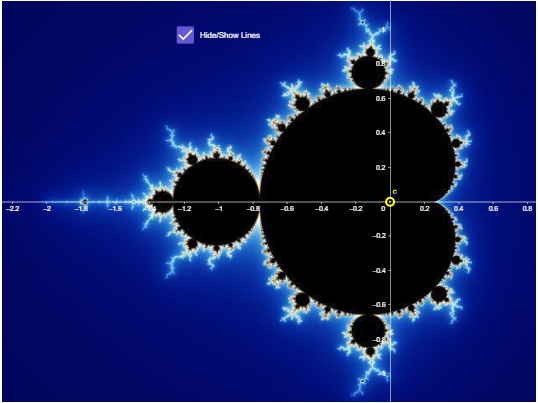
\includegraphics[width=0.5\linewidth]{image9.png}
\end{center}

% \protect\hypertarget{_Toc167901654}{}{}Abbildung 4: Veranschaulichung
% der Folge \(z_{n + 1} = z_{n}^{2}\) mit \(z_{0} = 0\) mittels
% GeoGebra (\url{https://www.geogebra.org/m/Npd3kBKn})

Diese Darstellung lässt vermuten, dass die Folge
\(\left( z_{n} \right)\) für \(z_{0} = 0\) gegen den Wert
\(a = 0\) konvergent ist, da an dieser Stelle ein Häufungspunkt zu
erkennen ist. Diese Vermutung muss nun untersucht werden. Betrachtet man
zunächst die ersten Folgenglieder:
\begin{align*}
z_{0} &= 0 \\
z_{1} &= 0^{2} + 0 = 0 + 0 = 0\\
z_{2} &= 0^{2} + 0 = 0 + 0 = 0\\
z_{3} &= 0^{2} + 0 = 0 + 0 = 0
\end{align*}
Wie anhand der ersten Folgenglieder erkennbar ist, wird nur der Wert 0
angenommen, die Folge konvergiert also gegen 0. Dieses Beispiel ist
trivial und kann somit einen guten Einstieg in die Thematik der
Folgenkonvergenz bieten. Zudem kann so gezeigt werden, dass
„\(\infty\)`` nicht zwingend das letzte Glied einer Folge ist. Außerdem
kann in diesem Zusammenhang thematisiert werden, dass der Grenzwert
erreicht werden kann, aber nicht muss.

\section{Beispiel für Divergenz ($c=-1$)}

Man betrachte die Folge \(\left( z_{n} \right)\) mit der
Bildungsvorschrift \(z_{n + 1} = z_{n}^{2} + c\) mit
\(n \in \mathbb{N}_{0}\) und \(c =  - 1\), der Startwert ist dabei
\(z_{0} =  - 1\). Diese wird mittels eines GeoGebra Applets
veranschaulicht.

\begin{center}
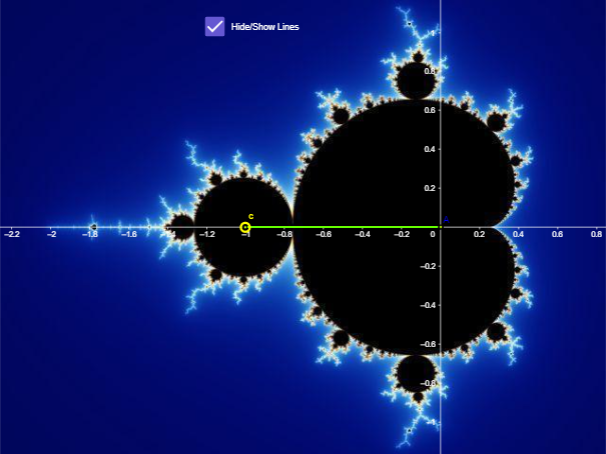
\includegraphics[width=0.5\linewidth]{image10.png}
\end{center}

% \protect\hypertarget{_Toc167901655}{}{}Abbildung 5: Darstellung der
% Folge \(z_{n + 1} = z_{n}^{2}–1\) mit \(z_{0} =  - 1\)
% mittels GeoGebra (\url{https://www.geogebra.org/m/Npd3kBKn})

Diese Darstellung lässt vermuten, dass die Folge
\(\left( z_{n} \right)\) für \(z_{0} =  - 1\) divergent ist, da
sowohl bei \(-\)1 als auch bei 0 ein Häufungspunkt zu erkennen ist. Da
die bildliche Darstellung allein aber nicht ausreicht, muss diese
Vermutung nun genauer untersucht werden. Betrachtet man zunächst die
ersten Folgenglieder:
\begin{align*}
z_{0} &=  - 1 \\
z_{1} &= ( - 1)^{2} - 1 = 1 - 1 = 0 \\
z_{2} &= 0^{2} - 1 = 0 - 1 =  - 1 \\
z_{3} &= ( - 1)^{2} - 1 = 1 - 1 = 0 \\
z_{4} &= 0^{2} - 1 = 0 - 1 =  - 1 \\
z_{5} &= ( - 1)^{2} - 1 = 1 - 1 = 0
\end{align*}
Betrachtet man die ersten Folgenglieder, so ist eindeutig erkennbar,
dass die Folge abwechselnd die beiden Werte 0 und \(-1\) annimmt. Sie
ist somit divergent.

Wie dieses Beispiel zeigt, kann die Mandelbrot-Menge nicht nur zur
Veranschaulichung der Konvergenz, sondern auch zur Visualisierung von
Divergenz eingesetzt werden. Außerdem bietet es sich an, in diesem
Zusammenhang auf Häufungspunkte einzugehen.

\section{Weiteres Beispiel einer Konvergenz ($c=0.25$)}

Ein weniger triviales Beispiel für eine konvergente Folge ist
\(\left( z_{n} \right)\) mit der Bildungsvorschrift
\(z_{n + 1} = z_{n}^{2} + c\) mit \(n \in \mathbb{N}_{0}\) und
\(c = 0.25\), der Startwert ist dabei \(z_{0} = 0.25\). Auch
diese Folge wird mit einem GeoGebra Applet visualisiert.

\begin{center}
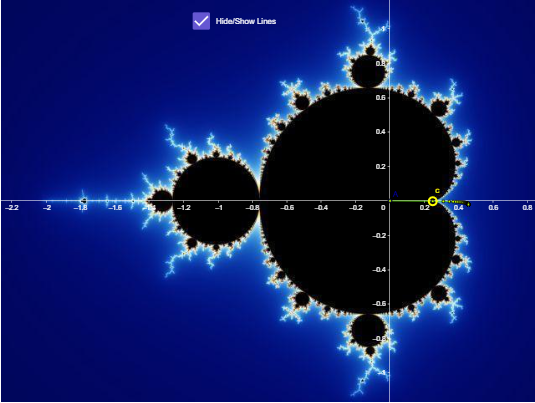
\includegraphics[width=0.5\linewidth]{image11.png}
\end{center}

% \protect\hypertarget{_Toc167901656}{}{}Abbildung 6: Visualisierung der
% Folge \(z_{n + 1} = z_{n}^{2} + 0.25\) mit \(z_{0} = 0.25\)
% mittels GeoGebra (\url{https://www.geogebra.org/m/Npd3kBKn})

Diese Darstellung lässt vermuten, dass die Folge
\(\left( z_{n} \right)\) für \(z_{0} = 0.25\) konvergent ist, auch
wenn der Grenzwert \(a\) nicht direkt abgelesen werden kann.

\subsection*{Beweis}

Betrachtet man zunächst die ersten Folgenglieder:
\begin{align*}
z_{0} &= 0.25\\
z_{1} &= {0.25}^{2} + 0.25 = 0.0625 + 0.25 = 0.3125\\
z_{2} &= {0.3125}^{2} + 0.25 = 0.3476...\\
z_{3} &= {0.3476...}^{2} + 0.25 = 0.3708...\\
z_{4} &= {0.3708...}^{2} + 0.25 = 0.3875...\\
z_{5} &= {0.3875...}^{2} + 0.25 = 0.4001...\\
z_{6} &= {0.4001...}^{2} + 0.25 = 0.4101...\\
      &\vdotswithin{=} % das fehlt von Roboto?
\end{align*}

Diese Werte lassen keine eindeutige Vermutung über das Konvergenz- oder
Divergenzverhalten zu, da die Folge monoton steigend zu seien scheint.
Abbildung 6 deutet aber stark auf eine Konvergenz hin.

Daher nehmen wir an, dass die Folge \(\left( z_{n} \right)\) für
\(z_{0} = 0.25\) einen Grenzwert \(a\) besitzt, wenn
\(n \rightarrow \infty\) und versuchen nun, dies zu beweisen.

Wie nehmen an, dass die Folge \(\left( z_{n} \right)\) für
\(z_{0} = 0.25\) einen Grenzwert \(a\) besitzt, wenn
\(n \rightarrow \infty\).

Dann muss gelten:

\[z_{n + 1} = z_{n}^{2} + 0.25\overset{\Leftrightarrow}{\binom{n \rightarrow \infty}{\left( z_{n} \right) \rightarrow a}}a = a^{2} + 0.25 \Longleftrightarrow 0 = a^{2} - a + 0.25\]

Also gilt für den Grenzwert \(a\):

\[a = \frac{1}{2} \pm \sqrt{\left( \frac{1}{2} \right)^{2} - 0.25} = \frac{1 \pm \sqrt{0}}{2} = \frac{1}{2}\]

Das heißt, wir haben den möglichen Grenzwert \(a = 0.5\) der Folge
\(\left( z_{n} \right)\) für \(z_{0} = 0.25\) gefunden.

Um zu beweisen, dass \(a = 0.5\) wirklich der Grenzwert der Folge
ist, zeigen wir, dass \(z_{n}\) monoton steigend und von \(a = 0.5\)
beschränkt wird, das heißt, dass \(z_{n} \leq 0.5\) für alle
\(n\mathbb{ \in N}\).

\begin{enumerate}
\item
  Monotonie:

\begin{itemize}
\item Induktionsanfang (\(n = 0\)):
\[z_{0} = 0.25 \leq z_{1} = 0.3125\]
\item Induktionsschritt:
\begin{itemize}
\item Induktionsannahme: \(\forall n \in \mathbb{N}:z_{n + 1} \geq z_{n}\)
\item Induktionsbehauptung:
\(\forall n \in \mathbb{N}:z_{n + 2} \geq z_{n + 1}\)
\end{itemize}
\[z_{n + 2} = z_{n + 1}^{2} + 0.25 \geq z_{n + 1}\text{\textcolor{red}{WARUM?}}\]
\end{itemize}
Also ist die Folge \(z_{n}\) monoton steigend.

\item
  Beschränktheit: \(z_{n} \leq 0.5\) für alle \(n\mathbb{ \in N}\)
\begin{itemize}
\item Induktionsanfang (\(n = 0\)):
\[z_{0} = 0.25 \leq 0.5\]
\item Induktionsschritt:
\begin{itemize}
\item Induktionsannahme: \(\forall n \in \mathbb{N}:z_{n} \leq 0.5\)
\item Induktionsbehauptung:
\(\forall n \in \mathbb{N}:z_{n + 1} \leq 0.5\)
\end{itemize}
\[z_{n + 1} = z_{n}^{2} + 0.25 \leq {0.5}^{2} + 0.25 \leq 0.5\]
\end{itemize}
Also ist die Folge \(z_{n}\) beschränkt durch 0.5.
\end{enumerate}

Aus der Monotonie und der Beschränktheit der Folge \(z_{n}\) folgt also,
dass \(a = 0.5\) wirklich der Grenzwert der Folge \(z_{n}\) ist.
\hfill\blacksquare

% Eine Visualisierung dieses Beispiels zeigt die Konvergenz besonders
% schön, da der Verlauf der Folgenglieder gut zu sehen ist. Die Konvergenz
% ist aber nicht trivial und zeigt die Notwendigkeit von Beweisen.

\section{$c=-0.5$ ist Element der Mandelbrot-Menge}

Ein weniger einfaches Beispiel für eine konvergente Folge ist
\(\left( z_{n} \right)\) mit der Regel \(z_{n + 1} = z_{n}^{2} + c\) mit
\(n \in \mathbb{N}_{0}\) und \(c =  -0.5\), der Startwert ist dabei
\(z_{0} =  -0.5\). Auch diese Folge kann mit einem GeoGebra Applet
veranschaulicht werden.

\begin{center}
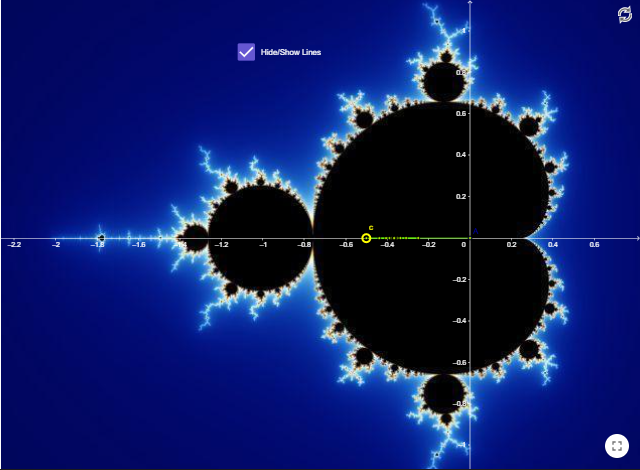
\includegraphics[width=0.5\linewidth]{image12.png}
\end{center}

% \protect\hypertarget{_Toc167901657}{}{}Abbildung 7: Visualisierung der
% Folge \(z_{n + 1} = z_{n}^{2} - 0.5\) mit \(z_{0} =  - 0.5\)
% mittels GeoGebra (\url{https://www.geogebra.org/m/Npd3kBKn})

Diese Abbildung legt die Vermutung nahe, dass die Folge konvergent ist
und der Grenzwert \(a\) zwischen \(-0.5\) und \(-0.25\) liegt.


Betrachtet man zunächst die ersten Folgenglieder:

\begin{align*}
z_{0} &=  - 0.5\\
z_{1} &= ( - {0.5)}^{2} - 0.5 = 0.25 - 0.5 =  -0.25\\
z_{2} &= ( - {0.25)}^{2} - 0.5 =  -0.4375\\
z_{3} &= {( - 0.4375)}^{2} - 0.5 =  -0.3085...\\
z_{4} &= {( - 0.3085...)}^{2} - 0.5 =  -0.4047...\\
z_{5} &= {( - 0.4047...)}^{2} - 0.5 =  -0.3361...\\
z_{6} &= {( - 0.3361...)}^{2} - 0.5 =  -0.3869...
\end{align*}

Diese Werte liegen zwischen \(-0.5\) und \(-0.25\) und scheinen sich
einem Wert zwischen diesen beiden anzunähern, wobei die Werte für
\(n \in \mathbb{N}_{g}\) beginnend bei \(-0.5\) monoton wachsend
gegen einen Grenzwert und die Werte für \(n \in \mathbb{N}_{u}\)
beginnend bei \(-0.25\) monoton fallend gegen diesen Grenzwert zu
streben scheinen.

Wie nehmen an, dass die Folge \(\left( z_{n} \right)\) für
\(z_{0} =  -0.5\) einen Grenzwert \(a\) besitzt, wenn
\(n \rightarrow \infty\).

Dann muss $(z_n)\to a$ gelten, falls $z_{n + 1} = z_{n}^{2} - 0.5$ und $n\to\infty$:

\[a = a^{2} - 0.5 \Longleftrightarrow 0 = a^{2} - a - 0.5\]

Also gilt für den Grenzwert \(a\):

\[a = \frac{1}{2} \pm \sqrt{\left( \frac{1}{2} \right)^{2} + 0.5} = \frac{1}{2} \pm \sqrt{\frac{3}{4}} = \frac{1 \pm \sqrt{3}}{2}.\]

Das heißt, die Fixpunkte der rekursiv definierten Folge und somit die
möglichen Grenzwerte der Folge \(\left( z_{n} \right)\) für
\(z_{0} =  - 0.5\) sind \(a = \frac{1 \pm \sqrt{3}}{2}\).

Nun prüfen wir, ob einer der beiden Fixpunkte wirklich Grenzwert der
Folge ist. Dazu betrachten wir zwei Teilfolgen \(x_{n}\) und \(y_{n}\)
von \(z_{n}\).

Seien \(x_{n}\) und \(y_{n}\) Teilfolgen von \(z_{n}\), wobei
\(n \in \mathbb{N}_{g}\) für \(x_{n}\) und
\(n \in \mathbb{N}_{u}\) für \(y_{n}\).

Betrachten wir die Folge \(x_{n}\).

\begin{align*}
x_{0} &= z_{0} =  -0.5\\
x_{1} &= z_{2} = z_{1}^{2} - 0.5 = (z_{0}^{2} - 0.5)^{2} - 0.5 = x_{0}^{4} - {x_{0}}^{2} - 0.25\\
x_{2} &= z_{4} = z_{3}^{2} - 0.5 = (z_{2}^{2} - 0.5)^{2} - 0.5 = x_{1}^{4} - {x_{1}}^{2} - 0.25\\
x_{3} &= z_{6} = z_{5}^{2} - 0.5 = (z_{4}^{2} - 0.5)^{2} - 0.5 = x_{2}^{4} - {x_{2}}^{2} - 0.25\\
&\vdotswithin{=} \\
x_{n + 1} &= x_{n}^{4} - x_{n}^{2} - 0.25
\end{align*}

Um Konvergenz der Folge \(x_{n}\) beweisen zu können, müssen wir zeigen,
dass \(x_{n}\) sowohl beschränkt als auch monoton im Intervall
\(- 0.5\leq x_{n} \leq  - 0.25\) ist. Das zeigen wir durch
vollständige Induktion über $n$.

z.~z.~\(x_{n}\) ist beschränkt und monoton.

\begin{itemize}
\item Induktionsanfang (\(n = 0\)):
\[- 0.5 \leq  - 0.5 \leq  - 0.25\]
und
\[{- 0.4375 = x_{1} > x}_{0} =  -0.5\]
\item Induktionsschritt:
\begin{itemize}
\item Induktionsannahme:
\(\forall n \in \mathbb{N}: -0.5\leq x_{n} \leq  - 0.25\)
und \(x_{n + 1} > x_{n}\)
\item Induktionsbehauptung:
\(\forall n \in \mathbb{N} -0.5\leq x_{n + 1} \leq  - 0.25\)
und \(x_{n + 2} > x_{n + 1}\)

\begin{enumerate}
\item  Monotonie:
z.~z.~für \(-0.5\leq x_{n} \leq  -0.25\) ist
\(x_{n + 1} > x_{n}\) bzw. \(x_{n + 1} - {x}_{n} > 0\)

Sei \(f(x) = x^{4} - x^{2} - x - 0.25\).
Wir untersuchen nun, wann \(f(x) > 0\) gilt. Hierzu lösen wir die
Ungleichung im Intervall \(- 0.5\leq x_{n} \leq  - 0.25\):
\begin{align*}
f(x) &> 0\\
x^{4} - x^{2} - x - 0.25 &> 0\\
4x^{4} - 4x^{2} - 4x - 1 &> 0\\
4x^{4} - 4x^{3} + 4x^{3} - 2x^{2} - 4x^{2} + 2x^{2} - 2x - 2x - 1&> 0\\
2x^{2} \cdot (2x^{2} - 2x - 1) + 2x \cdot (2x^{2} - 2x - 1) + 2x^{2} - 2x - 1 &> 0\\
(2x^{2} - 2x - 1) \cdot (2x^{2} + 2x + 1) &> 0
\end{align*}

Fallunterscheidung:

\begin{enumerate}
\item
  1.~Fall:
\[2x^{2} - 2x - 1 > 0\;\land\;2x^{2} + 2x + 1 > 0\]
Wir lösen zunächst die Ungleichung \(2x^{2} - 2x - 1 > 0\):
\[2x^{2} - 2x - 1 > 0\]
Da die Nullstellen der Gleichung $2x^{2} - 2x - 1 = 0$
\begin{align*}
x_{1,2} &= \frac{1}{2} \pm \sqrt{\left( \frac{1}{2} \right)^{2} + 0.5}
= \frac{1}{2} \pm \sqrt{\frac{3}{4}} = \frac{1 \pm \sqrt{3}}{2}
\end{align*}
sind, gilt
\begin{align*}
2x^{2} - 2x - 1 = 2 \cdot \left(x - \frac{1 + \sqrt{3}}{2}\right) \cdot \left(x - \frac{1 - \sqrt{3}}{2}\right) &> 0\\
\left(x - \frac{1 + \sqrt{3}}{2}\right) \cdot \left(x - \frac{1 - \sqrt{3}}{2}\right) &> 0
\end{align*}
d.~h.
\[x - \frac{1 + \sqrt{3}}{2} > 0 \;\land\; x - \frac{1 - \sqrt{3}}{2} > 0\]
oder
\[x - \frac{1 + \sqrt{3}}{2} < 0 \;\land\; x - \frac{1 - \sqrt{3}}{2} < 0\]
Also:
\[x > \frac{1 + \sqrt{3}}{2} \land x > \frac{1 - \sqrt{3}}{2}\]
oder
\[x < \frac{1 + \sqrt{3}}{2} \land x < \frac{1 - \sqrt{3}}{2}\]
Somit folgt für die Lösungsmenge:
\[x \in \left(  - \infty,\frac{1 - \sqrt{3}}{2} \right) \cup \left( \frac{1 + \sqrt{3}}{2},\infty \right)\]
Nun betrachten wir noch die zweite Ungleichung des 1.~Falls:
\[2x^{2} + 2x + 1 > 0\]
Diese Ungleichung ist für alle \(x\mathbb{ \in R}\) erfüllt.

Somit ist die Lösungsmenge für den 1.~Fall:

\[x \in \left(\left(  - \infty,\frac{1 - \sqrt{3}}{2} \right) \cup
\left( \frac{1 + \sqrt{3}}{2},\infty \right)\right) \cap x\in\mathbb{R}\]
Zusammengefasst:
\[x \in \left(  - \infty,\frac{1 - \sqrt{3}}{2} \right) \cup
\left( \frac{1 + \sqrt{3}}{2},\infty \right)\]
\item 2.~Fall:
\[2x^{2} - 2x - 1 < 0\;\land\;2x^{2} + 2x + 1 < 0\]
Die Berechnungen im 2. Fall sind analog zum ersten Fall. Es ergeben sich
folgende Lösungen:
\begin{itemize}
\item Für \(2x^{2} - 2x - 1 < 0\):
\[x \in \left( \frac{1 - \sqrt{3}}{2},\frac{1 + \sqrt{3}}{2} \right)\]
\item Und für \(2x^{2} + 2x + 1 < 0\):
\[x \in \varnothing\]
\end{itemize}
Somit insgesamt:
\[x \in \varnothing\]
\end{enumerate}
Die Vereinigung der Lösungsmengen der beiden Fälle ergibt folglich:
\[x \in \left(  - \infty,\frac{1 - \sqrt{3}}{2} \right) \cup \left( \frac{1 + \sqrt{3}}{2},\infty \right)\]
Somit ergibt sich für das untersuchte Intervall
\(- 0.5\leq x_{n} \leq  - 0.25\), dass die Funktion \(f\) im
Intervall
\(\left( - 0.5,\frac{1 - \sqrt{3}}{2} \right)\)
monoton steigend ist.
\item
  Beschränktheit: Angenommen \(- 0.5\leq x_{n} \leq  - 0.25\) gilt.

Wir betrachten:
\(x_{n + 1} = x_{n}^{4} - x_{n}^{2} -0.25\) für
\(x_{n} =  -0.5\) und \(x_{n} =  -0.25\) (Intervallgrenzen).

Für \(x_{n} =  -0.5\):
\(x_{n + 1} = (-0.5)^{4} - (-0.5)^{2} - 0.25 =  -0,4375\).

Für \(x_{n} =  -0.25\):
\(x_{n + 1} = ( -0.25)^{4} - ( -0.25)^{2} - 0.25 =  -0,3085...\)

Also gilt
\(\forall n \in \mathbb{N}: -0.5{\leq x}_{n + 1} \leq  -0.25\),
da die Folge \(x_{n}\) für
\(-0.5\leq x_{n} \leq  -0.25\) monoton steigend ist und
die Werte \({x}_{n + 1}\) innerhalb von
\(-0.5\leq x_{n + 1} \leq  -0.25\) liegen.

Insgesamt gilt also für \(x_{n}\), dass die Folge im Intervall
\(-0.5\leq x_{n} \leq  -0.25\) monoton wachsend und
beschränkt ist. Nach dem Monotonieprinzip gilt
also, dass \(x_{n}\) konvergiert. Der Grenzwert ist dabei
\(a = \frac{1 - \sqrt{3}}{2}\). Dieser kann aus der Lösung der
Gleichung \(x^{4} - x^{2} - x - 0.25 = 0\) ermittelt
werden.

\end{enumerate}
\end{itemize}
\end{itemize}

Betrachten wir die Folge \(y_{n}\).
\begin{align*}
y_{0} &= z_{1} =  -0.25\\
y_{1} &= z_{3} = z_{2}^{2} - 0.5 = (z_{1}^{2} - 0.5)^{2} - 0.5 = y_{0}^{4} - y_{0}^{2} - 0.25\\
y_{2} &= z_{5} = z_{4}^{2} - 0.5 = (z_{3}^{2} - 0.5)^{2} - 0.5 = y_{1}^{4} - y_{1}^{2} - 0.25\\
y_{3} &= z_{7} = z_{6}^{2} - 0.5 = (z_{6}^{2} - 0.5)^{2} - 0.5 = y_{2}^{4} - y_{2}^{2} - 0.25\\
&\vdotswithin{=}\\
y_{n + 1} &= y_{n}^{4} - y_{n}^{2} - 0.25
\end{align*}
Die Konvergenz der Folge \(y_{n}\) im Intervall
\(-0.5\leq y_{n} \leq  - 0.25\) beweisen wir, indem wir,
wie im Fall \(x_{n}\), zeigen, dass \(y_{n}\) sowohl beschränkt als auch
monoton ist. Hier verwenden wir ebenfalls eine vollständige Induktion
über $n$. Die Schritte dieses Beweises sind hierbei analog zum Beweis für
die Folge \(x_{n}\). Und auch der Grenzwert kann analog, durch lösen der
Gleichung \(y^{4} - y^{2} - y - 0.25 = 0\) ermittelt
werden und ist dabei \(a = \frac{1 - \sqrt{3}}{2}\).

Beide Teilfolgen \(x_{n}\) und \(y_{n}\) von \(z_{n}\) konvergieren also
gegen denselben Wert. Folglich ist die gesamte Folge \(z_{n}\)
konvergent gegen diesen Grenzwert \(a = \frac{1 - \sqrt{3}}{2}\).

\hfill\blacksquare

\section{Noch ein Beispiel einer Divergenz ($c=1$)}

Nicht alle reellen Zahlen sind Element der Mandelbrot-Menge, wie am
Beispiel von \(c = 1\) gezeigt werden kann. Ein weiteres Beispiel
für eine divergente Folge ist \(\left( z_{n} \right)\) mit der
Bildungsvorschrift \(z_{n + 1} = z_{n}^{2} + c\) mit
\(n \in \mathbb{N}_{0}\) und \(c = 1\), der Startwert ist dabei
\(z_{0} = 1\).

\subsection*{Beweis}

Betrachtet man zunächst die ersten Folgenglieder:

\begin{align*}
z_{0} &= 1\\
z_{1} &= 1^{2} + 1 = 1 + 1 = 2\\
z_{2} &= 2^{2} + 1 = 5\\
z_{3} &= 5^{2} + 1 = 26\\
z_{4} &= 26^{2} + 1 = 677\\
z_{5} &= 677^{2} + 1 = 458330\\
&\vdotswithin{=}
\end{align*}

Diese Werte deuten stark auf ein divergentes Verhalten der Folge hin.

Wir beweisen die Divergenz über das Minorantenkriterium für Folgen, d.~h.~%
wir betrachten eine Folge \(x_{n}\), die kleiner als \(z_{n}\) ist und
wenn diese Folge divergiert, folgt daraus, dass auch \(z_{n}\) divergent
ist.

Wir betrachten zunächst die Folge \(x_{n + 1} = x_{n}^{2}\) mit
\(x_{0} = 2\).

\begin{align*}
x_{0} &= 2\\
x_{1} &= 2^{2} = 4\\
x_{2} &= 4^{2} = 16\\
x_{3} &= 16^{2} = 256\\
&\vdotswithin{=}
\end{align*}

Die Folge \(x_{n}\) kann explizit angegeben werden durch
\(x_{n} = 2^{2^{n}}\).

Nun betrachten wir den Grenzwert der Folge \(x_{n}\):
\(\lim_{n \rightarrow \infty}x_{n} = \lim_{n \rightarrow \infty}2^{2^{n}} = \infty\).
\(x_{n}\) ist also divergent.

Nun vergleichen wir die Folgen \(x_{n}\) und \(z_{n}\). Für die ersten
Folgenglieder gilt, dass \(x_{n} > \) \(z_{n}\). Allerdings hat die
Rekursionsformel von \(z_{n}\) den zusätzlichen Term „+1``, wodurch die
Folge \(z_{n}\) ab einem bestimmten Wert größer als \(x_{n}\) wird, da
\(z_{n}\) schneller wächst. Somit gilt nach dem Minorantenkriterium für
Folgen, dass \(z_{n}\) divergent ist und folglich ist \(c = 1\) kein
Element der Mandelbrot-Menge. \hfill\blacksquare

Eine Visualisierung dieses Beispiels ist mit dem bisher genutzten
GeoGebra Applet nicht mehr möglich, da die Skalierung in diesem Applet
nicht ausreicht. Allerdings kann der Beweis dennoch durchgeführt werden.
% Auch dieses Beispiel eignet sich für die Universität, da Beweismethoden
% und Konzepte verwendet werden, die nicht unbedingt der Schulmathematik
% entsprechen. Zudem können Grenzen der Visualisierung thematisiert
% werden.


\nocite{*}
\bibliography{Literaturen}

\end{document}
